% Usa o estilo abntex2, configurando detalhes de formatação e hifenização.
\documentclass[
	12pt,				
	oneside,		
	a4paper,			
	english,			% Idioma adicional para hifenização.
	french,				% Idioma adicional para hifenização.
	spanish,			% Idioma adicional para hifenização.
	brazil				% O último idioma é o principal do documento.
	]{abntex2}



%%% Importação de pacotes. %%%

% Pacotes não documentados:
\usepackage{etex}
\reserveinserts{28}
\usepackage{colortbl}
\usepackage{framed}

\usepackage{longtable}
\usepackage{pdflscape}

% Usa a fonte Latin Modern.
\usepackage{lmodern}

% Seleção de códigos de fonte.
\usepackage[T1]{fontenc}

% Codificação do documento em Unicode.
\usepackage[utf8]{inputenc}

% Usado pela ficha catalográfica.
\usepackage{lastpage}

% Indenta o primeiro parágrafo de cada seção.
\usepackage{indentfirst}

% Controle das cores.
\usepackage[usenames,dvipsnames]{xcolor}

% Inclusão de gráficos.
\usepackage{graphicx}

% Inclusão de páginas em PDF diretamente no documento (para uso nos apêndices).
\usepackage{pdfpages}

% Para melhorias de justificação.
\usepackage{microtype}

% Citações padrão ABNT.
\usepackage[brazilian,hyperpageref]{backref}
\usepackage[alf]{abntex2cite}	
\renewcommand{\backrefpagesname}{Citado na(s) página(s):~}		% Usado sem a opção hyperpageref de backref.
\renewcommand{\backref}{}										% Texto padrão antes do número das páginas.
\renewcommand*{\backrefalt}[4]{									% Define os textos da citação.
	\ifcase #1
		Nenhuma citação no texto.
	\or
		Citado na página #2.
	\else
		Citado #1 vezes nas páginas #2.
	\fi}

% Pacotes não incluídos no template abntex2. 
% Podem ser comentados caso não queira utilizá-los.

% Inclusão de símbolos não padrão.
\usepackage{amssymb}
\usepackage{eurosym}

% Para utilizar \eqref para referenciar equações.
\usepackage{amsmath}

% Permite mostrar figuras muito largas em modo paisagem com \begin{sidewaysfigure} ao invés de \begin{figure}.
\usepackage{rotating}

% Permite customizar listas enumeradas/com marcadores.
\usepackage{enumitem}

% Permite inserir hiperlinks com \url{}.
\usepackage{bigfoot}
\usepackage{hyperref}

% Color control.
\usepackage[usenames,dvipsnames]{xcolor}

% Permite usar o comando \hl{} para evidenciar texto com fundo amarelo. Útil para chamar atenção a itens a fazer.
% O comando \phl é definido para que o professor evidencie texto com uma cor diferente para adicionar notas.
\usepackage{soulutf8}
\newcommand{\phl}[2][Peach]{{\sethlcolor{#1} \hl{#2}}}


% Permite usar o comando \hl{} para evidenciar texto com fundo amarelo. Útil para chamar atenção a itens a fazer.
\usepackage{soul}


% Permite inserir espaço em branco condicional (incluído no texto final só se necessário) em macros.
\usepackage{xspace}

% Permite incluir listagens de código com o comando \lstinputlisting{}.
\usepackage{listings}
\usepackage{caption}
\DeclareCaptionFont{white}{\color{white}}
\DeclareCaptionFormat{listing}{\colorbox{gray}{\parbox{\textwidth}{#1#2#3}}}
\captionsetup[lstlisting]{format=listing,labelfont=white,textfont=white}
\renewcommand{\lstlistingname}{Listagem}
\definecolor{mygray}{rgb}{0.5,0.5,0.5}
\lstset{
	basicstyle=\scriptsize,
	breaklines=true,
	numbers=left,
	numbersep=5pt,
	numberstyle=\tiny\color{mygray}, 
	rulecolor=\color{black},
	showstringspaces=false,
	tabsize=2,
    inputencoding=utf8,
    extendedchars=true,
    literate=%
    {é}{{\'{e}}}1
    {è}{{\`{e}}}1
    {ê}{{\^{e}}}1
    {ë}{{\¨{e}}}1
    {É}{{\'{E}}}1
    {Ê}{{\^{E}}}1
    {û}{{\^{u}}}1
    {ù}{{\`{u}}}1
    {â}{{\^{a}}}1
    {à}{{\`{a}}}1
    {á}{{\'{a}}}1
    {ã}{{\~{a}}}1
    {Á}{{\'{A}}}1
    {Â}{{\^{A}}}1
    {Ã}{{\~{A}}}1
    {ç}{{\c{c}}}1
    {Ç}{{\c{C}}}1
    {õ}{{\~{o}}}1
    {ó}{{\'{o}}}1
    {ô}{{\^{o}}}1
    {Õ}{{\~{O}}}1
    {Ó}{{\'{O}}}1
    {Ô}{{\^{O}}}1
    {î}{{\^{i}}}1
    {Î}{{\^{I}}}1
    {í}{{\'{i}}}1
    {Í}{{\~{Í}}}1
}

% Colorinlistoftodos package: to insert colored comments so authors can collaborate on the content.
\usepackage[colorinlistoftodos, textwidth=20mm, textsize=footnotesize]{todonotes}
\newcommand{\bruno}[1]{\todo[author=\textbf{Bruno},color=green!30,caption={},inline]{#1}}
\newcommand{\vitor}[1]{\todo[author=\textbf{Vítor},color=red!30,caption={},inline]{#1}}




%%% Definição de variáveis. %%%

\renewcommand{\imprimircapa}{%
	\begin{capa}%
		\center
		
		{\ABNTEXchapterfont\large\subtitulo{}}
		\vfill
		\begin{center}
			\ABNTEXchapterfont\bfseries\LARGE\imprimirtitulo
		\end{center}
		
		\vfill
		Registro de Alterações:
		\begin{table}[h]
			\centering
			\vspace{0.5cm}
			\begin{tabular}{|c|c|c|p{4.5cm}|}  \hline  \rowcolor[rgb]{0.8,0.8,0.8}
 				
 				Versão & Resposável & Data  & Alterações \\	\hline  
 				                            
				1.0 & Bruno Manzoli    & 10/09/2015  & \textit{versão inicial} \\ \hline 
				
				1.1 & Vítor E. Silva Souza    & 22/09/2015  & \textit{primeira revisão} \\ \hline 
				
				2.0 & Bruno Manzoli    & 08/10/2015  & \textit{correção e alterações} \\	\hline
				
				2.1 & Vítor E. Silva Souza & 12/11/2015 & \textit{segunda revisão} \\ \hline
				
				2.2 & Bruno Manzoli & 19/11/2015 & \textit{correção relatórios e RF} \\ \hline
				
				\versao	& Bruno Manzoli & 11/04/2016 & \textit{Junção dos documentos} \\ \hline
				 
			\end{tabular}
		\end{table}
		
		\vfill
		\large\imprimirlocal
		\linebreak
		\large\imprimirdata
		\vspace*{1cm}
	\end{capa}
}

\newcommand{\versao}{3.0}
\newcommand{\subtitulo}{Documento de Especificação de Requisitos}

\titulo{ SAE - Sistema de Acompanhamento de Egressos }
\autor{Bruno Manzoli do Nascimento}
\local{Vitória, ES}
\data{2015}

\instituicao{
  Universidade Federal do Espírito Santo -- UFES
  \par
  Centro Tecnológico
  \par
  Departamento de Informática}
\tipotrabalho{Monografia (PG)}







% Macros específicas do trabalho.
% (*) Inclua aqui termos que são utilizados muitas vezes e que demandam formatação especial.
% Os exemplos abaixo incluem i* (substituindo o asterisco por uma estrela) e Java com TM em superscript.
% Use sempre \xspace para que o LaTeX inclua espaço em branco após a macro somente quando necessário.
\newcommand{\istar}{\textit{i}$^\star$\xspace}
\newcommand{\java}{Java\texttrademark\xspace}
\newcommand{\latex}{\LaTeX\xspace}




%%% Configurações finais de aparência. %%%

% Altera o aspecto da cor azul.
\definecolor{blue}{RGB}{41,5,195}

% Informações do PDF.
\makeatletter
\hypersetup{
	pdftitle={\@title}, 
	pdfauthor={\@author},
	pdfsubject={\imprimirpreambulo},
	pdfcreator={LaTeX with abnTeX2},
	pdfkeywords={abnt}{latex}{abntex}{abntex2}{trabalho acadêmico}, 
	colorlinks=true,				% Colore os links (ao invés de usar caixas).
	linkcolor=blue,					% Cor dos links.
	citecolor=blue,					% Cor dos links na bibliografia.
	filecolor=magenta,				% Cor dos links de arquivo.
	urlcolor=blue,					% Cor das URLs.
	bookmarksdepth=4
}
\makeatother

% Espaçamentos entre linhas e parágrafos.
\setlength{\parindent}{1.3cm}
\setlength{\parskip}{0.2cm}



%%% Páginas iniciais do documento: capa, folha de rosto, ficha, resumo, tabelas, etc. %%%

% Compila o índice.
\makeindex















% Inicia o documento.
\begin{document}

% Retira espaço extra obsoleto entre as frases.
\frenchspacing


\begin{figure}[h]
  \centering
  
\includegraphics[scale=0.055]{figuras/brasao.jpg}
  \label{ppts3}
  \end{figure} 

% Capa do trabalho.
\imprimircapa





%%% Início da parte de conteúdo do documento. %%%
% Marca o início dos elementos textuais.
\textual
% Inclusão dos capítulos.
% (*) Para facilitar a organização, os capítulos foram divididos em arquivo separados e colocados dentro da.
% pasta capitulos/. Caso o aluno prefira trabalhar com um só arquivo, basta substituir os comandos \include 
% pelos conteúdos dos arquivos que estão sendo incluídos, excluindo a pasta capitulos/ em seguida.

\begingroup
\let\clearpage\relax
% ==============================================================================
% TCC - César Henrique Bernabé
% Capítulo 1 - Introdução
% ==============================================================================

\chapter{Introdução}
\label{sec-intro}

O avanço da tecnologia nas ultimas décadas permitiu que a complexidade das atividades realizadas por computadores se tornasse cada vez maior, demandando que projetos de sistemas de software passassem a abranger ainda mais os detalhes de domínio do ambiente em que os programas computacionais seriam executados ~\cite{andersson2009modeling,brun2009engineering}. Esse fator motivou estudos na área de modelagem e projeto de sistemas, fazendo com que novas pesquisas buscassem abranger os processos de projeto, construção e teste de software. 

Entretanto, para garantir a estabilidade dos sistemas, fazia-se uso majoritariamente da intervenção humana, o que rapidamente tornou-se inviável à medida que os sistemas cresciam para atender o aumento da demanda de novos usuários~\cite{andersson2009modeling}. Assim, a utilização de sistemas adaptativos vem tornando-se a solução mais viável e prática para a atual conjuntura do desenvolvimento de softwares. Além disso, o aumento do número de diferentes dispositivos e situações em que esses softwares podem ser executados faz com que eles passem a enfrentar uma grande diversidade de contextos (muitas vezes imprevisíveis) de execução, fundamentando ainda mais a pesquisa na área de softwares adaptativos~\cite{kephart2003vision}.

Sistemas adaptativos são dotados da capacidade de tomar decisões para se ajustar e se reconfigurar mediante mudanças de contexto, permitindo assim que os requisitos elicitados continuem a ser atendidos de forma satisfatória~\cite{souza2012requirement}. Entretanto, poucas soluções desse tipo consideram a modelagem das características adaptativas no sistema desde a fase de modelagem do mesmo. \zanshin~\cite{tesevitor} aparece como uma abordagem que baseia-se em modelos para projetar características adaptativas em sistemas por meio de novos tipos de requisitos, que definem o chamado ``ciclo de retroalimentação'', que operacionaliza a adaptação. Seguindo uma abordagem de Desenvolvimento Dirigido por Modelos, \zanshin apresenta um metamodelo que permite que modelos de sistemas sejam especificados de acordo com os requisitos do \framework.

Este trabalho encontra-se no contexto da pesquisa em torno da abordagem \zanshin, mais especificamente lidando com duas de suas limitações: (1) seu metamodelo atual não representa fielmente o conjunto de modelos desejados; e (2) não há uma ferramenta CASE que auxilie engenheiros de requisitos no uso da abordagem.



\section{Objetivos}
\label{sec-intro-objetivos}

Este trabalho possui dois objetivos principais: a reconstrução do metamodelo operacional do \zanshin e a criação de uma ferramenta gráfica usada para modelar sistemas adaptativos usando Engenharia de Requisitos Orientada a Objetivos (\textit{Goal-Oriented Requirements Engineering} ou \gore). O primeiro refere-se ao metamodelo de objetivos que é baseado em \textit{CORE} (\textit{Core Ontology for Requirements Engineering})~\cite{jureta2007core}, usado pelo framework para casar os requisitos do modelo de domínio específico com as instâncias dos elementos do metamodelo de \gore, e assim garantir que os objetivos do sistema estão sendo atendidos satisfatoriamente. Já a segunda atividade refere-se à ferramenta de modelagem de sistemas baseada nesse metamodelo operacional do \zanshin, usando sintaxe baseada em uma linguagem de especificação de modelos ontológicos conceituais conhecida como iStar~\cite{dalpiaz2016istar}. Para ambos os casos, foram utilizados os conceitos aprendidos ao longo do curso de Ciência da Computação. Dessa forma são objetivos específicos deste projeto:


\begin{itemize}
	
	\item Levantar as deficiências do metamodelo atual do \zanshin, identificando os pontos em que as relações entre os elementos deveriam ser modificadas para representarem mais fielmente as formalidades da Engenharia de Requisitos Orientada a Objetivos;
	
	\item Elaborar um metamodelo atualizado que, além de representar mais rigorosamente a hierarquia dos elementos \gore, também reflita as necessidades da arquitetura do \zanshin, como por exemplo as relações entre elementos;
	
	\item Modificar o código fonte do \textit{framework} para que o mesmo possa utilizar o novo metamodelo desenvolvido e executar o mecanismo de adaptações considerando esse novo metamodelo;
	
	\item Desenvolver uma ferramenta que permita ao usuário criar uma representação gráfica do modelo do sistema alvo e implementar, dentro dessa ferramenta, um módulo para converter o modelo gráfico representado para arquivos \xml que possam ser importados diretamente para o \zanshin;
	
	\item Apresentar os trabalhos desenvolvidos, juntamente com as perspectivas futuras de otimização de ambos os sistemas apresentados.

\end{itemize}


\section{Metodologia}
\label{sec-intro-metodologia}

O trabalho realizado compreendeu as seguintes atividades:


\begin{enumerate}
	
	\item \textit{Revisão Bibliográfica}: Estudo sobre Engenharia de Requisitos Orientada a Objetivos, Desenvolvimento Dirigido por Modelos e suas ferramentas, de publicações acadêmicas sobre \zanshin e sobre desenvolvimento de sistemas adaptativos;
	
	\item \textit{Estudo das Tecnologias:} Levantamento das tecnologias disponíveis para \textit{Eclipse Modeling Framework} (\emf) que permitam o desenvolvimento de editores gráficos dentro da plataforma \eclipse, de tecnologias que podem ser utilizadas para o desenvolvimento de editores gráficos e do código fonte do \zanshin (que também foi desenvolvido nessa plataforma);
	
	\item \textit{Elaboração do novo Metamodelo}: Nessa etapa o novo metamodelo a ser usado foi elaborado gradativamente a partir de informações obtidas dos documentos estudados e das discussões realizadas em reuniões com grupo de estudos de Engenharia de Requisitos na UFES;
	
	\item \textit{Adequação do \zanshin ao novo Metamodelo}: Após finalização do metamodelo, inicou-se processo de adequação do \framework para que o mesmo pudesse operar de acordo com a nova proposta, consistindo da modificação do código-fonte do \zanshin, bem como realização de testes de validação para garantir a consistência do novo metamodelo;
	
	\item \textit{Implementação da Ferramenta de Modelagem}: Uma primeira versão da ferramenta foi desenvolvida no contexto de trabalho de Iniciação Científica, entretanto a mesma usava o metamodelo antigo do \zanshin. Essa etapa consiste, portanto, no refatoramento da ferramenta gráfica que permite a modelagem de sistemas adaptativos seguindo as formalidades do novo metamodelo proposto para o sistema \zanshin, bem como a criação de módulo usando linguagem de transformação de modelos para texto, que permite a exportação do modelo desenvolvido nessa ferramenta para arquivo \xml adequado aos padrões do \framework;
	
	\item \textit{Redação da Monografia:} Escrita da monografia, etapa obrigatória do processo de elaboração do Projeto de Graduação. Para a escrita desta, foi utilizada a linguagem \textit{LaTeX}\footnote{LaTeX -- http://www.latex-project.org/} utilizando o template \textit{abnTeX}\footnote{abnTeX -- http://www.abntex.net.br} que atende os requisitos das normas da ABNT (Associação Brasileira de Normas Técnicas) para elaboração de documentos técnicos e científicos brasileiros. Para apoiar este processo, foi utilizado o aplicativo \textit{TeXstudio}.\footnote{www.texstudio.org}
	
\end{enumerate}


%%% Início de seção. %%%
\section{Organização do Texto}
\label{sec-intro-organizacao}

Este texto está dividido em quatro partes principais além desta introdução, que seguem:

\begin{itemize}
	\item \textbf{Capítulo \ref{sec-referencial} --} Referencial Teórico: apresenta discussão acerca de \gore e \mdd, focando na relação desses tópicos com sistemas adaptativos e com o processo de desenvolvimento da ferramenta \unagi. Ademais, é discutida a arquitetura do sistema \zanshin e suas características;
	
	\item \textbf{Capítulo \ref{sec-zanshin} --} Zanshin: nesse capitulo são apresentados os processos e decisões que levaram à elaboração do novo metamodelo do \zanshin, bem como as modificações decorrentes dessas modificações na arquitetura da plataforma;
	
	\item \textbf{Capítulo \ref{sec-unagi} --} Unagi: Nesse capítulo é abordado o processo de desenvolvimento da ferramenta \unagi e os pormenores da implementação de todos os módulos da mesma;
	
	\item \textbf{Capítulo \ref{sec-validacao} --} Revisão: é feita validação do metamodelo evoluído do \zanshin e da implementação da ferramenta \unagi;
	
	\item \textbf{Capítulo \ref{sec-conclusoes} --} Considerações Finais: apresenta as conclusões obtidas ao final deste trabalho, bem como as dificuldades encontradas e as perspectivas de trabalhos futuros para esse contexto.
\end{itemize}










\vspace*{2cm}

\chapter{Descrição do Propósito do Sistema}
\label{sec-proposito}


O Departamento de Informática da Universidade Federal do Espírito Santo (DI/Ufes) necessita de um sistema de informação para o acompanhamento dos alunos egressos, com o propósito estimular principalmente alunos do ensino médio pela área da informática, para isso os egressos forneceriam dados como área de atuação, faixa salarial, curso de pós-graduação realizados, possibilitando assim obter informações de perfil dos egressos e gerar relatórios estatísticos que ficariam disponíveis na Internet. 


\vspace*{2cm}

\chapter{Descrição do Minimundo}
\label{sec-minimundo}

O DI/Ufes deseja um sistema de informação para acompanhar seus alunos egressos dos cursos de graduação (Ciência da Computação e Engenharia de Computação) e de pós-graduação (Mestrado em Informática e Doutorado em Ciência da Computação). 

Para poder acessar o sistema, os egressos terão um pré-cadastro realizado por um administrador do sistema. Somente poderão ser pré-cadastrados ex-alunos que tenham se formado em algum curso oferecido pelo DI/Ufes. Para efetuar o pré-cadastro o administrador buscará os dados do egresso junto à Ufes, a saber: nome, data de nascimento, sexo, e-mail, identidade, CPF, naturalidade e nacionalidade. Também serão informados o curso em que o egresso se formou, o número de sua matrícula, o ano de ingresso e o ano de término. 

Assim que o pré-cadastro for realizado, o sistema deverá enviar um e-mail ao egresso com um link que o leva diretamente para uma página onde pode definir sua senha. Para aumentar a segurança, esta página solicita o CPF ou a matrícula do egresso para efetivar a definição de senha. Caso o egresso perca este e-mail, poderá receber outro, devendo para isso entrar no site e informar o seu CPF/matrícula, o sistema reconhecendo o egresso, enviará o e-mail.
 
Assim que for criada a senha, o sistema levará o egresso a uma página onde ele preencherá um formulário com os seguintes campos: faixa salarial, área de atuação, se atua na área em que se formou, nível de escolaridade e se reside no ES. Para cada nível de escolaridade deve dizer o título obtido, o ano, a instituição, o estado e o país.

O tempo médio exigido para o preenchimento deste formulário deve ser inferior a 5 minutos. A cada 2 anos o sistema deverá enviar um e-mail para que o usuário atualize esses dados, sendo armazenado o histórico dos mesmos.

Os egressos escolherão a sua área de atuação dentre as seguintes opções: empreendedor; funcionário público; funcionário privado; professor; ou pesquisador. E informarão se atuam em Informática, área afim ou área não correlata. Será perguntado se a formação acadêmica adquirida no curso da Ufes contribuiu para a sua atividade atual.

Os egressos escolherão a faixa salarial, dividida da seguinte forma: até 3 salários mínimos; de 3 a 5 salários mínimos; de 5 a 10 salários mínimos;  de 10 a 15 salários mínimos; de 15 a 20 salários mínimos; e acima de 20 salários mínimos. Poderão também optar por assuntos de interesse para recebimento de e-mail. A princípio os assuntos serão: Redes de Computadores e Sistemas Distribuídos; Computação de Alto Desempenho; Inteligência Computacional; Sistema de Informação; e Otimização. 

Egressos poderão postar depoimentos sobre o curso que realizaram. Esses depoimentos ficarão acessíveis a todos que acessarem o site, depois de serem avaliados e liberados pelo coordenador do curso a fim de evitar críticas gratuitas depreciativas. O egresso poderá optar por aparecer seu nome no depoimento ou se ele quer que fique anônimo. De um depoimento deseja-se saber a data de envio, sobre qual curso, o autor e o conteúdo. 

Assim como no caso dos depoimentos, os egressos também poderão mandar comentários ou sugestões sobre o curso que realizaram. Estes serão enviadas para o coordenador do curso para que possa respondê-los e também auxiliar em melhorias a serem feitas nos cursos. 

Administradores do sistema poderão cadastrar seminários, informando o assunto, o título, a data e horário, o local e o palestrante. Caso não tenha palestrante ainda, o administrador terá a opção de enviar um e-mail aos egressos convidando-os a serem o palestrante. Caso alguém responda ao chamado (por e-mail, externo ao sistema), o administrador terminaria o cadastro do seminário. Assim que a palestra estiver confirmada, o sistema enviará um e-mail para todos os egressos que tenham interesse pelo assunto, convidando-os para participarem. Os egressos também teriam a opção de sugerir um assunto em que tenham interesse em ser o palestrante. Neste caso o administrador confirmaria com ele e cadastraria o seminário no sistema.


\section{Relatórios}
\label{sec-minimundo:relatorio}

\noindent No site, ficarão disponíveis para consulta relatórios sobre dados estatísticos. Estes dados serão mostrados na forma de gráficos, assim os usuários poderão escolher um curso e optar pelos seguintes gráficos: 

\begin{itemize}
	
  	\item \textbf{Faixa Salarial:} mostra a porcentagem de egresso em cada faixa salarial.
  	
  	\item \textbf{Área de Atuação:} mostra a porcentagem de egresso em cada área: (Empreendedor), (Func. Público), (Func. Privado), (Professor) e (Pesquisador).
  	
  	\item \textbf{Atuação do Egresso:} mostra a porcentagem de egressos que atuam na área da informática, a porcentagem dos que atuam em áreas afins e a porcentagem dos que atuam em áreas não correlatas. 
  	
  	\item \textbf{Escolaridade:} mostra a porcentagem de egressos em cada nível de escolaridade. 
  	
  	\item \textbf{Reside no ES:} mostra a porcentagem de egressos que moram no Estado.
  	
  	\item \textbf{Sexo:} mostra a porcentagem de egressos do sexo masculino e feminino.
  	
  	
\end{itemize}
   
  Os usuários também poderão consultar todos os egressos, que serão mostrados na forma de lista.
\endgroup


\begin{landscape}


	\chapter{Requisitos de Usuário}
	\label{sec-requisitos}

	\noindent {\large Tomando por base o contexto do sistema, foram identificados os seguintes requisitos de usuário e regras de negócio:}
	
\newcounter{rfcount}
\renewcommand*\therfcount{RF-\arabic{rfcount}}
\newcommand*\RF{\refstepcounter{rfcount}\therfcount}
\setcounter{rfcount}{0}

 \begin{longtable}{|c|p{16.5cm}|c|p{2.3cm}|}
 			
			\caption{Requisitos Funcionais} \\ \hline \rowcolor[rgb]{0.8,0.8,0.8}
 					
 			Identificador &  Descrição  &  Prioridade   &  	Depende   \\ \hline	
 				
			\RF\label{rf-cadastro-Administrador} & O sistema deve permitir o cadastro de administradores, com as seguintes informações: nome, email, CPF e matricula. & Alta & {}\\ \hline  
			
			\RF\label{rf-cadastro-Egresso} & O sistema deve permitir o cadastro de egressos, abrangendo egressos dos cursos de graduação e de pós-graduação do DI/Ufes. & Alta & \ref{rf-cadastro-Administrador}, \ref{rn-aluno-formado-DI}\\ \hline
			
			\RF\label{rf-gerenciamento-curso}  &  O sistema deve permitir o gerenciamento de cursos, incluindo as informações de nome, codigo e quem é o coordenador do curso. & Alta & \ref{rf-cadastro-Administrador} \\ \hline 
			
			\RF\label{rf-gerenciamento-assuntos-interesse} &  O sistema deve permitir o gerenciamento de assuntos de interesse. & Alta & \ref{rf-cadastro-Administrador} \\\hline 
					
			\RF\label{rf-gerenciamento-seminario}  & O sistema deve permitir o gerenciamento de seminários, armazenando informações como palestrante, o assunto, a data, horário e conteúdo. & Alta & \ref{rf-cadastro-Administrador}, \ref{rf-cadastro-Egresso}, \ref{rf-gerenciamento-assuntos-interesse}\\ \hline 
			
			\RF\label{rf-email-cadastro-egresso} & O sistema deve enviar email automaticamente aos egressos assim que forem pré-cadastrados, para que possam realizar a definição de senha e finalizar o cadastro. & Alta & 	\ref{rf-cadastro-Administrador},  \ref{rf-cadastro-Egresso} \\ \hline
			
			
			\RF\label{rf-novo-email-cadastro}  & O sistema deve permitir que o egresso, caso este perca o email de cadastro, entre no site e informe o seu CPF/Matricula, sendo reconhecido receberá um novo email. & Alta & \ref{rf-cadastro-Administrador},  \ref{rf-cadastro-Egresso} \\ \hline  
			
			\RF\label{rf-coordenador-responder-comentario}  &  O coordenador de um curso deve poder responder comentários. & Média & \ref{rf-cadastro-Administrador}, \ref{rf-cadastro-Egresso}, \ref{rf-gerenciamento-curso}, \ref{rf-gerenciamento-comentario} \\ \hline
					
			\RF\label{rf-coordenador-avaliar-depoimento}  &  O coordenador de um curso deve poder avaliar depoimentos, autorizando ou não a divulgação no site. & Média & \ref{rf-cadastro-Administrador}, \ref{rf-cadastro-Egresso}, \ref{rf-gerenciamento-curso}, \ref{rf-gerenciamento-depoimento} \\ \hline
					
			
			
			
			\RF\label{rf-gerenciamento-depoimento} & O sistema deve permitir que egressos enviem depoimentos sobre os cursos realizados no DI, armazenando informações como autor, conteúdo, curso, data de envio e se será anônimo. & Alta & \ref{rf-cadastro-Administrador}, \ref{rf-cadastro-Egresso}, \ref{rf-gerenciamento-curso} \\ \hline 
					
			\RF\label{rf-gerenciamento-comentario}  & O sistema deve permitir que os egressos enviem sugestões sobre os cursos que realizaram no DI, armazenando informações como o autor, o conteúdo, o curso e a data de envio. & 	Alta &  	\ref{rf-cadastro-Administrador}, \ref{rf-cadastro-Egresso}, \ref{rf-gerenciamento-curso} \\ \hline 
					
			\RF\label{rf-email-atualizacao-dados}  & O sistema deve enviar um email automaticamente aos egressos a cada 2 anos, a fim de solicitar aos egressos a atualização de seus dados. & 	Média & \ref{rf-cadastro-Administrador}, \ref{rf-cadastro-Egresso} \\ \hline 
					
			\RF\label{rf-gerar-relatorio}  & O sistema deve gerar relatórios estatísticos conforme a seção 3.1, permitindo sua consulta por qualquer usuário. & Alta & \ref{rf-cadastro-Administrador}, \ref{rf-cadastro-Egresso}, \ref{rf-gerenciamento-curso} \\ \hline 
					
			\RF\label{rf-egresso-atualizar-dados} & O egresso deve poder atualizar seus dados. & Alta &  \ref{rf-cadastro-Administrador}, \ref{rf-cadastro-Egresso} \\\hline 
			
			\RF\label{rf-egresso-elencar-assuntos-interesse}  & O egresso deve poder elencar seus assuntos de interesse. & Média & \ref{rf-cadastro-Administrador}, \ref{rf-cadastro-Egresso} \\ \hline 
					
			\RF\label{rf-egresso-palestrante}  & O egresso deve poder se voluntariar como palestrante e sugerir o assunto. & Média & \ref{rf-cadastro-Administrador}, \ref{rf-cadastro-Egresso}, \ref{rf-gerenciamento-seminario} \\ \hline  
			
			\RF\label{rf-consulta-depoimento}  & O sistema deve permitir a consulta de depoimentos por qualquer usuário. & Alta &  \ref{rf-cadastro-Egresso}, \ref{rf-coordenador-avaliar-depoimento}, \ref{rf-gerenciamento-depoimento}\\ \hline  
 
 
\end{longtable}







\newcounter{rncount}
\renewcommand*\therncount{RN-\arabic{rncount}}
\newcommand*\RN{\refstepcounter{rncount}\therncount}
\setcounter{rncount}{0}

\begin{longtable}{|c|p{16.5cm}|c|p{2.3cm}|}
			
			\caption{Regras de Negócio} \\ \hline \rowcolor[rgb]{0.8,0.8,0.8}
 			
 			Identificador & 	Descrição  &  Prioridade    & Depende  \\ \hline	
					
			\RN\label{rn-aluno-formado-DI}  & Só poderão se cadastrar no sistema alunos que se formaram em pelo menos um curso oferecido pelo DI, a saber : Ciência da Computação, Engenharia da Computação, Mestrado em Informática e Doutorado em Ciência da Computação & Alta & 	\\ \hline 
					
			\RN\label{rn-depoimento-curso}  & Egressos só poderão postar depoimento, comentar e sugerir sobre curso que tenha realizado.  & Alta &  \\ \hline 
				 
\end{longtable}
	


\newcounter{rnfcount}
\renewcommand*\thernfcount{RNF-\arabic{rnfcount}}
\newcommand*\RNF{\refstepcounter{rnfcount}\thernfcount}
\setcounter{rnfcount}{0}


\begin{longtable}{|c|p{12.5cm}|p{3.1cm}|c|c|}
	
			\caption{Requisitos Não Funcionais}\\ \hline \rowcolor[rgb]{0.8,0.8,0.8}
 					
 			Identificador &	Descrição  & Categoria  & Escopo  & Prioridade   \\ \hline		
					
			\RNF\label{rnf-Portabilidade}  & A ferramenta deve estar disponível como uma aplicação Web, acessível a partir dos principais navegadores disponíveis no mercado. & Portabilidade & 	Sistema  &	Alta \\	\hline 
					
			\RNF\label{rnf-facilidade-aprendizado}  & A ferramenta dever ser de aprendizado fácil, não sendo necessário nenhum treinamento especial para seu uso.  & Facilidade de Aprendizado  & Sistema &	Média   \\ \hline 
					
			\RNF\label{rnf-facilidade-operacao}  & A ferramenta deve ser de fácil operação, não sendo necessário uso contínuo para uma boa operação do sistema.  &	Facilidade de Operação  & Sistema &	Alta  \\ 	\hline 
					
			\RNF\label{rnf-seguranca-acesso}  & O sistema deve controlar o acesso as funcionalidades.  &	Segurança de acesso  &  Sistema 	 &	Alta  \\ \hline 
					
			\RNF\label{rnf-eficiencia-tempo}  & O tempo para o preenchimento do cadastro pelo egresso deve ser inferior a cinco minutos.  &	Eficiência em relação ao tempo  & Funcionalidade	 &	Alta  \\ 	\hline 
					
			\RNF\label{rnf-interoperabilidade}  & O sistema deve estar integrado a um sistema de correio eletrônico de modo que seja possível o envio de email automaticamente. &	Interoperabilidade & Funcionalidade & Alta  \\ \hline 
										
			\RNF\label{rnf-reusabilidade}  & O desenvolvimento do sistema deve explorar o potencial de reutilização de componentes, tanto no que se refere ao desenvolvimento com reúso quanto ao desenvolvimento para reúso.  & Reusabilidade  &	Sistema & Média  \\\hline 
				
\end{longtable}	
\end{landscape}

\chapter{ Identificação de Subsistemas}
\label{sec-subsistemas}

A Figura~\ref{figura-subsistema} mostra os subsistemas identificados no contexto do presente projeto, os quais são descritos na tabela abaixo.




\begin{figure}[h]
  \centering
  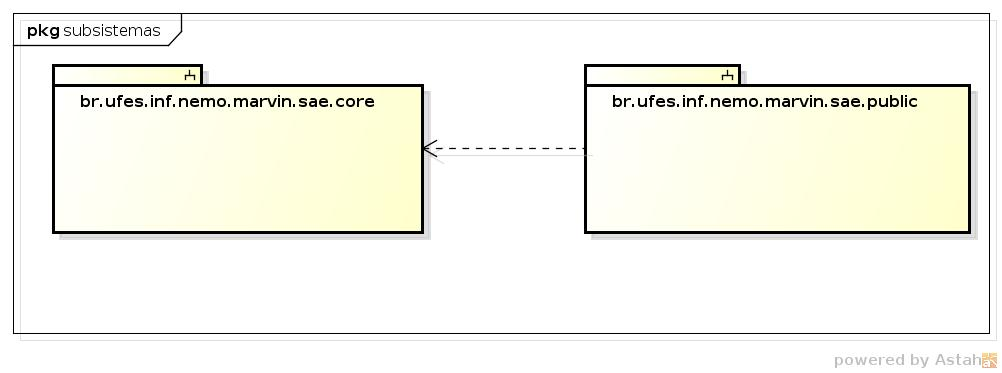
\includegraphics[width=1\textwidth]{figuras/fig-projeto-diagrama-pacotes}
  \caption{Diagrama de Pacotes e os Subsistemas Identificados.}
  \label{figura-subsistema}
\end{figure} 





\begin{table}[h]
	\centering	
	\vspace{0.5cm}
	
	\begin{tabular}{|p{3cm}|p{12cm}|}  \hline \rowcolor[rgb]{0.8,0.8,0.8}
	
 		Subsistema & Descrição \\\hline 
 		                             
		Core & Envolve toda a funcionalidade relacionada com o administrador do sistema, abrangendo controle de Séminarios, Cursos, Assuntos de interesse, envio de email automático e pré-cadastro de egresso. \\\hline
		                              
		Public & Envolve toda a funcionalidade relacionada com consultas a serem realizadas no site, e com as interações que os egressos poderão fazer, tais como cadastrar depoimentos e sugestões. \\\hline 
		
	\end{tabular}
	\caption{ Subsistemas}	
\end{table}


\chapter{Modelo de Casos de Uso}
\label{sec-caso-de-uso}

\newcounter{uccount}                                      \renewcommand*\theuccount{UC-\arabic{uccount}}
\newcommand*\UC{\refstepcounter{uccount}\theuccount}      \setcounter{uccount}{0}

O modelo de casos de uso visa capturar e descrever as funcionalidades que um sistema deve prover para os atores que interagem com o mesmo. Os atores identificados no contexto deste projeto estão descritos na tabela~\ref{tabela-atores}.

\begin{table}[h]
	\centering \vspace{0.5cm} \caption{ Atores}
	\begin{tabular}{|p{3cm}|p{12cm}|} \hline \rowcolor[rgb]{0.8,0.8,0.8}
 		Ator & Descrição \\\hline                              
		Administrador & Profissional da Ufes responsável pela parte administrativa do sistema. \\\hline   
		Coordenador & É um administrador responsável por um curso, avaliando depoimentos e sugestões enviadas pelos egressos. \\\hline                              
		Egresso & Ex-alunos da Ufes que tenham se formado em algum curso oferecido pelo DI/Ufes. \\\hline                              
		Visitante & Qualquer pessoa que acessar o site. \\\hline 		 
	\end{tabular}
	\label{tabela-atores}	
\end{table}



A Figura~\ref{figura-caso-de-uso-atores} apresenta o diagrama de herança entre os atores do sistema, de modo que essas heranças não serão mostradas nos outros diagramas para evitar a poluição visual.

\begin{figure}[h!]
	\centering
	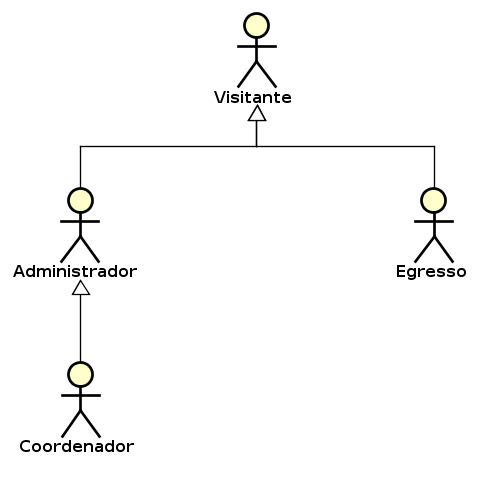
\includegraphics[width=0.5\textwidth]{figuras/atoresHeranca}
 	\caption{Diagrama de Herança dos Atores.}
 	\label{figura-caso-de-uso-atores}
\end{figure}


A seguir, são apresentados os diagramas de casos de uso e descrições associadas, organizados por subsistema.


\newpage
\section{Subsistema Core}

A Figura~\ref{figura-caso-de-uso-core} apresenta o diagrama de casos de uso do subsistema Core.

\begin{figure}[h!]
	\centering
	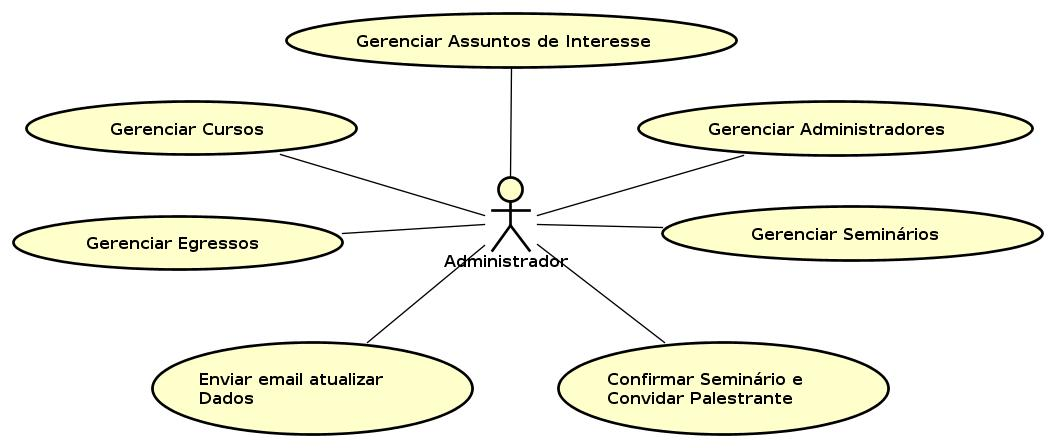
\includegraphics[width=1\textwidth]{figuras/casodeuso-core}
 	\caption{Diagrama de Casos de Uso do Subsistema Core.}
 	\label{figura-caso-de-uso-core}
\end{figure}
 
 A seguir, são apresentadas as descrições de cada um dos casos de uso identificados. Os casos de uso cadastrais de baixa complexidade, envolvendo inclusão, alteração, consulta e exclusão, são descritos na tabela~\ref{tabela-core-cadastrais}.


\newpage
\begin{table}[h]
	\centering  \vspace{0.5cm} 	\footnotesize 
	\caption{Casos de Uso Cadastrais}
	\begin{tabular}{|c|c|c|p{6cm}|c|c|} \hline  \rowcolor[rgb]{0.8,0.8,0.8}
 				
 		Id & Nome  &  Ações  &  Observações & Requisitos   & Classes  \\ 	\hline \hline	
 		
 		{}    &    {}    &   I   &    Informar: nome, email, matricula e CPF. Será criada uma senha padrão, e assim que o administrador fizer o primeiro acesso, o sistema solicitará a atualização da mesma.  &   {}   &   {}    \\\cline{3-4}
 		{}  &   Gerenciar    &   A   &   {}   &    {}   &    {}  \\ \cline{3-4}
 		\UC\label{uc-administrador}  &  Administradores  &  C  &   {}    &   RF-1  &   Administrador    \\\cline{3-4}
 	    {}   &  {}   &    E    &    Não é permitido excluir um administrador que é coordenador de um curso.   &  {}  &  {} \\ \hline \hline
 		
 		
 		
 		\rowcolor[rgb]{0.97,0.97,0.97}
 		{}   &  {}   &  I  &   Informar: nome, código e coordenador (deve ser escolhido dentre os administradores cadastrados).   &  {}   &  {}    \\ \cline{3-4} \rowcolor[rgb]{0.97,0.97,0.97}
 		{} &   Gerenciar   &   A   &   {}   &    {}  &    {}   \\ \cline{3-4} \rowcolor[rgb]{0.97,0.97,0.97}
 		\UC\label{uc-curso} &    Cursos   &  C  &  {}  &  RF-3  &  Curso \\ \cline{3-4} \rowcolor[rgb]{0.97,0.97,0.97} 
 		{}    &    {}     &   E   &    Não é permitido excluir um curso que tenha egressos associados.  &  {}   & {} \\ \hline \hline
 		  
 		  
 		  
 		          
 		{}     &   {}    &   I   &    Informar: nome.     &   {}   &    {}    \\ \cline{3-4}
 		{}  &   Gerenciar   &   A   &   {}      &   {}    &    Assunto de   \\\cline{3-4}
 		\UC\label{uc-assunto}  &    Assuntos de   &    C   &    {}     &  RF-4  &    Interesse   \\\cline{3-4}
 		{} & interesse & E & Não é permitido excluir um assunto que tenha seminários associados. & {} & {} \\ \hline \hline
 		
 		
 		
 		\rowcolor[rgb]{0.97,0.97,0.97}
 		{} & {} & {} & Informar: nome, email, CPF, data de nascimento, identidade, sexo, naturalidade e nacionalidade. & {} & {} \\ \rowcolor[rgb]{0.97,0.97,0.97} 
 		{} & Gerenciar  &  I  & O sistema ao registrar o egresso  &  RF-2  &  Egresso,   \\  \rowcolor[rgb]{0.97,0.97,0.97}
 		\UC\label{uc-egresso}  & Egressos  &  {}   &  deve enviar um email para o mesmo.  &  RF-6   &    {}     \\ \cline{3-4} \rowcolor[rgb]{0.97,0.97,0.97}
 		{}  &  {}   &  A  &   {}    &  RN-1 &    Curso Realizado   \\\cline{3-4} \rowcolor[rgb]{0.97,0.97,0.97}
 		{}  &  {}   &  C  &   {}    &   RF-7   &    {}   \\\cline{3-4} \rowcolor[rgb]{0.97,0.97,0.97}
 		{}  &  {}   &  E  &   Não é permitido excluir egressos.   &  {}   &  {}  \\ \hline \hline
 		
 		
 		
		{}  &  {}  &  I  &  Informar: titulo, palestrante, data, local e assunto de interesse.  &  {}  &  {}  \\ \cline{3-4}
 		{} & {}  &  A  &  Caso o seminário já tenha sido confirmado e enviado email, o sistema deve enviar um email aos egressos informandos as alterações. & {} & {} \\ \cline{3-4}
 		\UC\label{uc-seminario}   &  Gerenciar   &    C   &    {}     &  RF-5   &    Seminário   \\ \cline{3-4}
 		{}    &    Seminários   &  E  &  Caso o seminário já tenha sido confirmado e enviado email, o sistema deve enviar um email aos egressos informandos a exclusão do seminário.  &  {}   &  {}   \\ \hline 
 		 		
 		 		
	\end{tabular}
	\label{tabela-core-cadastrais}
\end{table}




\newpage
\begin{flushright}    \textbf{Descrição de Caso de Uso}   \end{flushright}         
\noindent  \textbf{Projeto:} \imprimirtitulo  \\ 
\textbf{Identificador do Caso de Uso:} \UC\label{uc-seminario} \\ 
\textbf{Caso de Uso:} Confirmar Seminário e Convidar Palestrante \\
\noindent \textbf{Descrição Sucinta:} Este caso de uso é responsável por confirmar a ocorrência de seminários e por convidar egressos para se apresentarem como palestrantes.\\

\begin{table}[h]
	\centering    \vspace{0.5cm}     \footnotesize
	\caption{Fluxos de Eventos Normais}
	\begin{tabular}{|p{2.3cm}|p{1.8cm}|p{10.7cm}|} \hline  \rowcolor[rgb]{0.8,0.8,0.8}
 					
 		Nome do Fluxo & Precondição & Descrição  \\ \hline		
		
		Confirmar & {} & 1. O administrador informa o seminário a ser confirmado.  \\
		Seminário & {} & 2. O sistema envia email a todos os egressos que tenham interesse naquele assunto.\\ \hline 
			
		Convidar & {} & 1. O administrador informa o seminário sem palestrante.  \\
		Palestrante & {} & 2. O sistema envia email a todos os egressos que tenham interesse naquele assunto, convidando-os a serem o palestrante.\\ \hline 
		
		
		Voluntariar & {} & 1. O egresso informa o assunto e voluntaria-se como palestrante.  \\
		Palestrante & {} & 2. O sistema envia um email para informar o administrador.\\ \hline 
		
	\end{tabular}	
\end{table}

	\begin{table}[h]
		\centering 	\vspace{0.5cm}    \footnotesize
		\caption{Fluxos de Eventos Variantes}
		\begin{tabular}{|p{4.3cm}|p{3.5cm}|p{7.0cm}|}    \hline  \rowcolor[rgb]{0.8,0.8,0.8}
 		
 			Fluxo Relacionado &  Variante  &  Descrição    \\	\hline		
		
			Voluntariar Palestrante/  & 2 - O envio de email      & 2a - O sistema envia um email para o usuário   \\ 
			Confirmar Seminário / 	  & retorna um erro.			&  que instalou o sistema informando do erro. \\
			Convidar Palestrante     &{}              & 3 - O sistema retorna uma mensagem de erro ao usuário. \\\hline
		
		\end{tabular}
	\end{table}	
	
	

\noindent  \textbf{Requisitos Relacionados:} RF-5, RF-16     \\ \textbf{Classes Relacionadas:} Seminário. 





\newpage
\begin{flushright}    \textbf{Descrição de Caso de Uso}   \end{flushright} 
\noindent \textbf{Projeto:} \imprimirtitulo \\
\textbf{Identificador do Caso de Uso:} \UC\label{uc-email-atualizar-dados}\\ 
\textbf{Caso de Uso:} Enviar email atualizar dados \\
\noindent \textbf{Descrição Sucinta:} Este caso de uso é responsável enviar para os egressos a cada 2 anos um email solicitando a atualização de seus dados.\\

\begin{table}[h]
	\centering 	\vspace{0.5cm} 	\footnotesize
	\caption{Fluxos de Eventos Normais}
	\begin{tabular}{|p{2.3cm}|p{1.1cm}|p{11.4cm}|} \hline  \rowcolor[rgb]{0.8,0.8,0.8}
 					
 		Nome do Fluxo & Precond. & Descrição  \\ \hline		
	
		Enviar email & {} & 1. O sistema verifica se o último pedido de atualização tem mais de 2 anos. \\ 
		
		{} & {} & 2. O administrador sendo alertado pelo sistema, envia email a todos o egressos. \\ \hline
		
		
				
	\end{tabular}	
\end{table}


	\begin{table}[h]
		\centering 	\vspace{0.5cm}    \footnotesize
		\caption{Fluxos de Eventos Variantes}
		\begin{tabular}{|p{3.8cm}|p{4cm}|p{7.0cm}|}    \hline  \rowcolor[rgb]{0.8,0.8,0.8}
 		
 			Fluxo Relacionado &  Variante  &  Descrição    \\	\hline		
		
			Enviar  		& 2 - O envio de email      & 2a - O sistema envia um email para o usuário   \\ 
			email		& retorna um erro.			&  que instalou o sistema informando do erro. \\
			{}    		&{}              			& 3 - O sistema retorna uma mensagem de erro ao usuário. \\\hline
		
		\end{tabular}
	\end{table}	

\noindent  \textbf{Requisitos Relacionados:} RF-12   %  \\ \textbf{Classes Relacionadas:} 












\newpage
\section{Subsistema Public}

A Figura~\ref{figura-caso-de-uso-public}  apresenta o diagrama de casos de uso do subsistema Public.

\begin{figure}[h!]
  \centering
  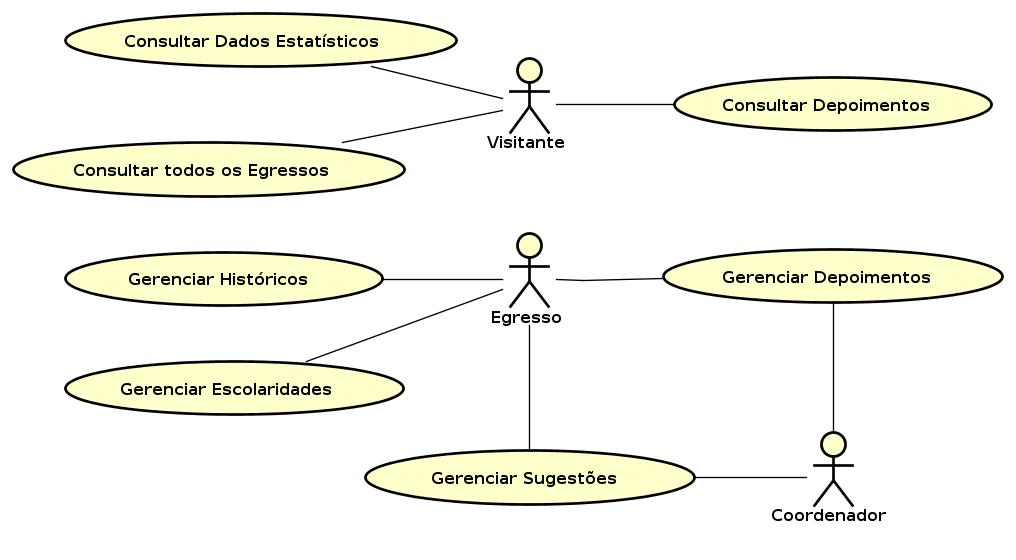
\includegraphics[width=1\textwidth]{figuras/casodeuso-public.jpg}
  \caption{Diagrama de Casos de Uso do Subsistema Public.}
  \label{figura-caso-de-uso-public}
\end{figure} 


Os casos de uso cadastrais de baixa complexidade, envolvendo inclusão, alteração, consulta e exclusão, são descritos na tabela~\ref{tabela-public-cadastrais}.

\begin{table}[h]
	\centering  \vspace{0.5cm} 	\footnotesize 
	\caption{Casos de Uso Cadastrais}
	\begin{tabular}{|c|c|c|p{6cm}|c|c|} \hline  \rowcolor[rgb]{0.8,0.8,0.8}
 				
 		Id & Nome  &  Ações  &  Observações & Requisitos   & Classes  \\ 	\hline 
 		
 		{}    &    {}    &   I   &    Informar: titulo, ano, intituição, estado e o país.  &   {}   &   {}    \\\cline{3-4}
 		\UC\label{uc-escolaridade}  &   Gerenciar    &   A  , C   &   {}   &    RF-14   &    Escolaridade  \\ \cline{3-4}
 		{}  & Escolaridades  &  E  &   {}    &   {}  &   {}  \\ \hline 
 		
 		{}    &    {}    &   I   &    Informar: faixa salarial, area de atuação, se atua na area de formação, o nível de escolaridade e se reside no Espirito Santo .  &   {}   &     \\\cline{3-4}
 		\UC\label{uc-historico}  &   Gerenciar    &   A  , C   &   {}   &    RF-14   &  Histórico      \\ \cline{3-4}
 		{}  & Histórico   &  E  &   {}    &   {}  &   do Egresso  \\ \hline 
 		
	\end{tabular}
	\label{tabela-public-cadastrais}
\end{table}




\newpage
Os casos de uso de consulta mais abrangente que as consulta a um único objeto, mas ainda de baixa complexidade, estão descritos na tabela~\ref{tabela-public-consulta}.

\begin{table}[h]
	\centering  \vspace{0.5cm} 	\footnotesize 
	\caption{Casos de Uso de Consulta}
	\begin{tabular}{|c|c|p{8cm}|c|c|} \hline  \rowcolor[rgb]{0.8,0.8,0.8}
 				
 		Id & Nome   &  Observações & Requisitos   & Classes  \\ 	\hline	
 		
 		{}  &  {}  &   As consultas aos egressos poderão ser feitas de forma  & {}   & {}    \\ 
 		{} &  Consultar   & geral onde serão mostrado todos os egressos, ou por  & {} & {} \\ 
 	    \UC\label{uc-consulta-todos-egresso}  &  Todos  & curso onde serão mostrados apenas os egressos que  & RF-13 & Egresso \\	
 	    {}  &  Egressos   &  formaram naquele curso, será exibido na tela para ao usuário o nome do egresso, o curso que realizou, o ano de inicio e o ano de termino.   & {}   & {}  \\	\hline
 	    
 	    
 	    
 	    {} &  {}  &  As consultas aos depoimentos poderão ser realizadas   & {}   & {}    \\ 
 		{} &  Consultar & de forma geral onde serão mostrados todos os  & {} & {} \\ 
 	    \UC\label{uc-consulta-depoimento} & Depoimento & depoimentos, ou por curso onde serão mostrados & RF-17 & Depoimento \\	
 	    {} & {}  & apenas depoimentos sobre o curso escolhido, será exibido na tela o conteúdo, o autor e a data de postagem. & {} & {} \\	\hline
 	    
 	     				
	\end{tabular}
	\label{tabela-public-consulta}
\end{table}




\newpage
\begin{flushright}    \textbf{Descrição de Caso de Uso}   \end{flushright}         
\noindent \textbf{Projeto:} \imprimirtitulo  \\
\textbf{Identificador do Caso de Uso:} \UC\label{uc-seminario} \\
\textbf{Caso de Uso:} Consultar dados Estatísticos \\
\noindent \textbf{Descrição Sucinta:} Este caso de uso é responsável por gerar relatórios com dados estatísticos sobre o perfil dos egressos.\\

\begin{table}[h]
	\centering \vspace{0.5cm} \footnotesize
	\caption{Fluxos de Eventos Normais}
	\begin{tabular}{|p{2.3cm}|p{1.8cm}|p{10.7cm}|} \hline  \rowcolor[rgb]{0.8,0.8,0.8}
 					
 		Nome do Fluxo & Precondição & Descrição  \\ \hline		
					
		Gerar    & {} & 1. O visitante informa o curso.  \\
		relatório    & {} & 2. O visitante informa o tipo de relatório: faixa salarial, atuação, escolaridade, entre outros (vide Documento de Especificação de Requisitos, seção 3.1).\\ 
        {} & {} & 3. O sistema gera o gráfico e mostra ao visitante.\\	\hline 
				
	\end{tabular}
\end{table}

\noindent  \textbf{Requisitos Relacionados:} RF-13       \\ \textbf{Classes Relacionadas:} Egresso, Histórico do Egresso.





\newpage
\begin{flushright}    \textbf{Descrição de Caso de Uso}   \end{flushright} 
\noindent \textbf{Projeto:} \imprimirtitulo \\
\textbf{Identificador do Caso de Uso:} \UC\label{uc-sugestao}\\ 
\textbf{Caso de Uso:} Gerenciar Sugestões \\
\noindent \textbf{Descrição Sucinta:} Este caso de uso é responsável gerenciar as sugestões enviadas pelos egressos.\\

\begin{table}[h]
	\centering 	\vspace{0.5cm} 	\footnotesize
	\caption{Fluxos de Eventos Normais}
	\begin{tabular}{|p{2.3cm}|p{1.8cm}|p{10.7cm}|} \hline  \rowcolor[rgb]{0.8,0.8,0.8}
 					
 		Nome do Fluxo & Precondição & Descrição  \\ \hline		
	
		Incluir nova  & {} & 1. O egresso informa o conteúdo da sugestão e o curso. \\ 
		Sugestão & {} & 2. O sistema preenche os campos data e autor. \\
		{} & {} & 3. O sistema envia um email ao coordenador do curso, informando da sugestão. \\ \hline
		
		Responder  & {} & 1. O coordenador seleciona a sugestão. \\ 
		Sugestão & {} & 2. O coordenador informa a resposta. \\
		{} & {} & 3. O sistema envia um email ao egresso autor da sugestão, com a resposta do coordenador. \\ \hline
				
	\end{tabular}	
\end{table}

\noindent  \textbf{Requisitos Relacionados:} RF-8, RF-11       \\ \textbf{Classes Relacionadas:} Sugestão










\newpage
\begin{flushright}    \textbf{Descrição de Caso de Uso}   \end{flushright} 
\noindent \textbf{Projeto:} \imprimirtitulo \\
\textbf{Identificador do Caso de Uso:} \UC\label{uc-depoimento}\\ 
\textbf{Caso de Uso:} Gerenciar Depoimentos \\
\noindent \textbf{Descrição Sucinta:} Este caso de uso é responsável gerenciar os depoimentos enviados pelos egressos.\\

\begin{table}[h]
	\centering 	\vspace{0.5cm} 	\footnotesize
	\caption{Fluxos de Eventos Normais}
	\begin{tabular}{|p{2.3cm}|p{1.8cm}|p{10.7cm}|} \hline  \rowcolor[rgb]{0.8,0.8,0.8}
 					
 		Nome do Fluxo & Precondição & Descrição  \\ \hline		
	
		Incluir novo & {} & 1. O egresso informa o conteúdo, se é anônimo e o curso. \\ 
		Depoimento & {} & 2. O sistema preenche os campos data e autor. \\
		{} & {} & 3. O sistema envia um email ao coordenador do curso, informando de um depoimento pendente. \\ \hline
		
		Avaliar  & {} & 1. O coordenador seleciona o depoimento pedente. \\ 
		Depoimento & {} & 2. O coordenador informa se liberado ou não liberado. \\\hline
				
		Alterar  & {} & 1. O egresso seleciona o depoimento. \\ 
		Depoimento & {} & 2. O egresso informa os novos dados. \\
		{} & {} & 3. O sistema envia um email ao coordenador do curso, informando de um depoimento pendente. \\ \hline
		
		Excluir   & {} & 1. O egresso seleciona o depoimento. \\ 
		Depoimento & {} & 2. O egresso confirma a exclusão. \\
		{} & {} & 3. O sistema exclui o depoimento. \\ \hline
				
	\end{tabular}	
\end{table}

\begin{table}[h]
	\centering 	\vspace{0.5cm}    \footnotesize
	\caption{Fluxos de Eventos Variantes}
	\begin{tabular}{|p{2.3cm}|p{4.8cm}|p{7.7cm}|}    \hline  \rowcolor[rgb]{0.8,0.8,0.8}
 		
 		Fluxo Relacionado &  Variante  &  Descrição    \\	\hline		
		
		Avaliar    & 2 - O coordenador avaliar como   & 2a - O sistema envia um email para o egresso,  \\ 
		Depoimento & não liberado & informando para refazer seu depoimento. \\\hline
		
	\end{tabular}
\end{table}

\noindent  \textbf{Requisitos Relacionados:} RF-9, RF-10     \\ \textbf{Classes Relacionadas:} Depoimento










\chapter{Modelo Estrutural}
\label{sec-modelo-estrutural}

O modelo conceitual estrutural visa capturar e descrever as informações (classes, associações e atributos) que o sistema deve representar para prover as funcionalidades descritas na seção anterior. A seguir, são apresentados os diagramas de classes de cada um dos subsistemas identificados no contexto deste projeto. Na seção~\ref{sec-dicionario} – Dicionário de Projeto – são apresentadas as descrições das classes, atributos e operações presentes nos diagramas apresentados nesta seção.


\section{Subsistema Core}

A Figura~\ref{figura-core-classe} apresenta o diagrama de classes do subsistema Core.

\begin{figure}[h]
  \centering
  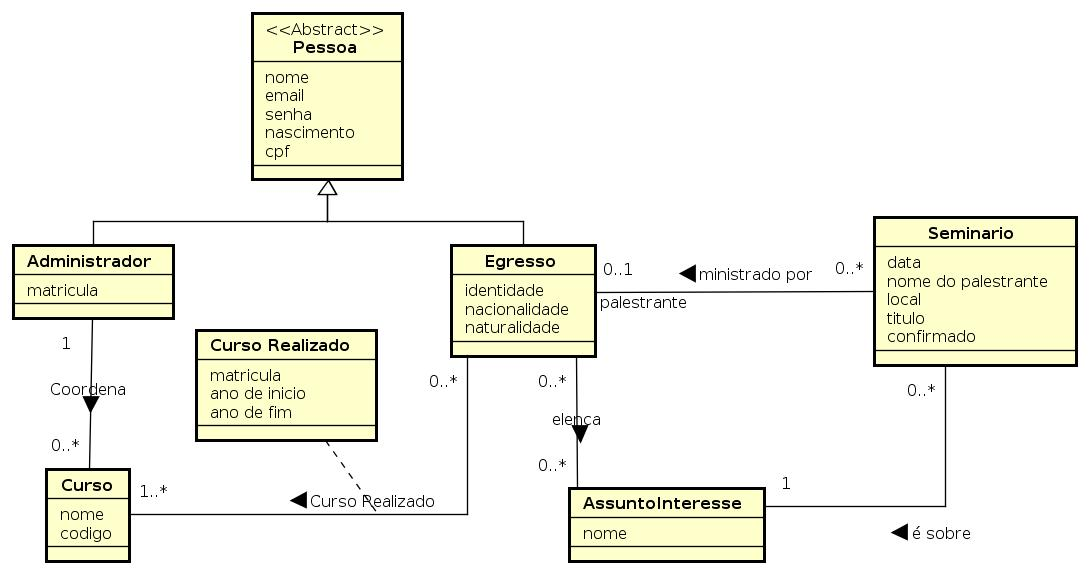
\includegraphics[width=1\textwidth]{figuras/diagrama-classe-core}
  \caption{Diagrama de Classes do Subsistema Core.}
  \label{figura-core-classe}
\end{figure} 


\newpage

\section{Subsistema Public}


A Figura~\ref{figura-public-classe} apresenta o diagrama de classes do subsistema Public.

\begin{figure}[h]
  \centering
  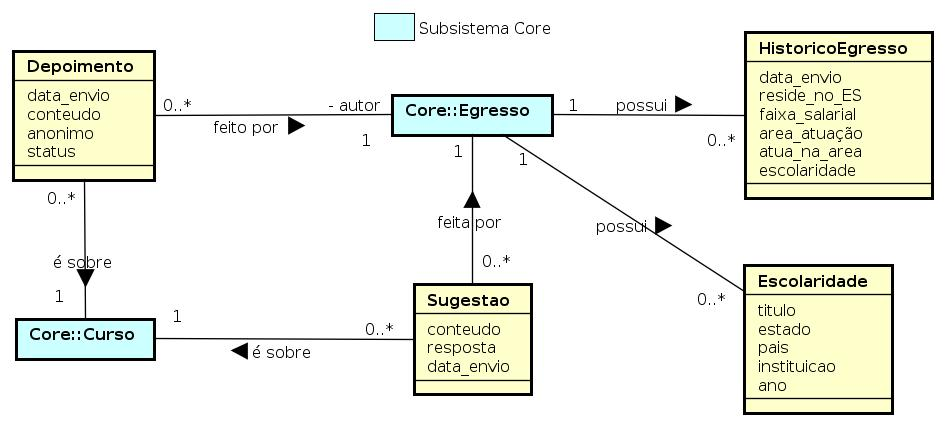
\includegraphics[width=1\textwidth]{figuras/diagrama-classe-public.jpg}
  \caption{Diagrama de Classes do Subsistema Public.}
  \label{figura-public-classe}
\end{figure} 
\newpage



\chapter{Modelo Dinâmico}
\label{sec-modelo-dinamico}

O modelo dinâmico visa capturar o comportamento dinâmico do sistema. A seguir, são
apresentados os diagramas de estados e o diagrama de atividades elaborados no contexto deste
projeto.


\section{Diagramas de Estados}


A Figura~\ref{figura-estado-depoimento} apresenta o diagrama de estados da classe Depoimento do subsistema Public.

\begin{figure}[h]
  \centering
  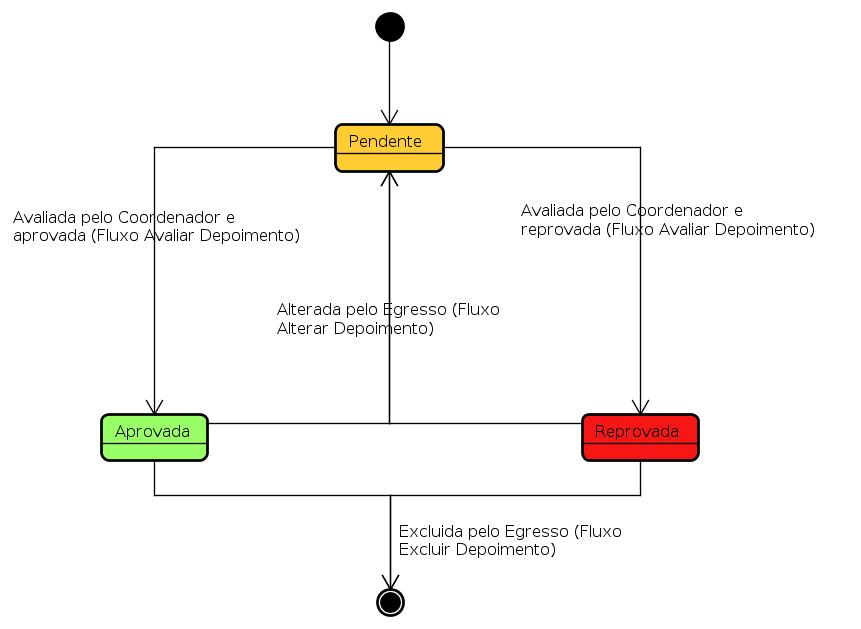
\includegraphics[scale=0.45]{figuras/estado-depoimento.jpg}
  \caption{Diagrama de Estados da Classe Depoimento.}
  \label{figura-estado-depoimento}
\end{figure}


\chapter{Dicionário de Projeto}
\label{sec-dicionario}
\setcounter{table}{0}

Esta seção apresenta as definições das classes (e seus atributos), servindo como um glossário do projeto. As definições são organizadas por subsistema. Vale destacar que eventuais operações que estas classes vierem a ter não são listadas e descritas nesta fase do projeto.


\section{Classes}

%%%%%       CLASSE EGRESSO        %%%%%%%%%%%%%%%%%%%%%%%%%%%%%%%%%%%%%%%%%%
\subsection{Egresso} \label{Egresso}
\begin{table}[h!]
	\footnotesize
	\begin{tabular}{|p{2.6cm}|c|c|p{7.8cm}|}   \hline \rowcolor[rgb]{0.8,0.8,0.8}
		
		%\multicolumn{4}{|c|}{ \textbf{Egresso}} \\ \hline \rowcolor[rgb]{0.95,0.95,0.95}
 		
 		\textbf{Propriedade} & \textbf{Tipo} & \textbf{Obrigatório?} & \centerline{\textbf{Descrição}} \\\hline  
 		                            
		nome & Texto & x & Nome completo do egresso. \\\hline  	
		
		data-nascimento & Data & x & Data de nascimento do egresso. \\\hline	
 		
		sexo & Caractere & x & Sexo do egresso. \\\hline 
		
		email & Texto & x & Email do egresso. \\\hline
		
		senha & Texto & x & Senha do egresso. \\\hline
		                             
		identidade & Texto & x & Número de RG do egresso. \\\hline
		
		cpf & Texto & x & Número de CPF do egresso. \\\hline
		
		naturalidade & Texto & & Naturalidade do egresso. \\\hline
		
		nacionalidade & Texto & & Nacionalidade do egresso. \\\hline
		
	\end{tabular}	
\end{table}


%%%%%       CLASSE EGRESSO-HISTORICO        %%%%%%%%%%%%%%%%%%%%%%%%%%%%%%%%%%%%%%%%%%
\subsection{Histórico do Egresso} \label{Histórico-do-Egresso}
\begin{table}[h!]
	\footnotesize
	\begin{tabular}{|p{2.6cm}|c|c|p{7.8cm}|}   \hline \rowcolor[rgb]{0.8,0.8,0.8}
	
		%\multicolumn{4}{|c|}{ \textbf{Histórico do Egresso}} \\ \hline \rowcolor[rgb]{0.95,0.95,0.95}
		
 		\textbf{Propriedade} & \textbf{Tipo} & \textbf{Obrigatório?} & \centerline{\textbf{Descrição}} \\\hline  	
	
 		data-envio & Data & x & Data de envio dos dados pelo egresso. \\\hline
		                      
		faixa-salarial & Enumerado & x & Faixa onde se encontra a renda do egresso. \\\hline
		
		area-atuacao & Enumerado & x & Área onde o egresso atua profissionalmente. \\\hline
		
		escolaridade & Enumerado & x & Nível de escolaridade do Egresso. \\\hline
		
		atua-na-area & Booleano & x & Se o egresso atua na área em que se formou. \\\hline		
		
		reside-ES & Booleano & x & Se o egresso reside no estado do Espirito Santo. \\\hline	
			
	
	\end{tabular}	
\end{table}


%%%%%       CLASSE ESCOLARIDADE        %%%%%%%%%%%%%%%%%%%%%%%%%%%%%%%%%%%%%%%%%%
\subsection{Escolaridade} \label{Escolaridade}
\begin{table}[h!]
	\footnotesize
	\begin{tabular}{|p{2.6cm}|c|c|p{7.8cm}|}   \hline \rowcolor[rgb]{0.8,0.8,0.8}
	
		%\multicolumn{4}{|c|}{ \textbf{Escolaridade}} \\ \hline \rowcolor[rgb]{0.95,0.95,0.95}
		
 		\textbf{Propriedade} & \textbf{Tipo} & \textbf{Obrigatório?} & \centerline{\textbf{Descrição}} \\\hline  	
	
 		titulo & Enum & x & Titulo da graduação adiquirida. \\\hline
		
		estado & Texto & x & Nome do estado onde foi realizado. \\\hline   
 		                      
		país & Texto & x & Nome do país onde foi realizado. \\\hline
		
		ano & Data & x & Ano de conclusão. \\\hline
		
		instituição & Texto & x & Nome da instituição onde foi realizado. \\\hline	
		
			
		
	\end{tabular}	
\end{table}

\newpage

%%%%%       CLASSE CURSO        %%%%%%%%%%%%%%%%%%%%%%%%%%%%%%%%%%%%%%%%%%
\subsection{Curso} \label{Curso}
\begin{table}[h!]
	\footnotesize
	\begin{tabular}{|p{2.6cm}|c|c|p{7.8cm}|}   \hline \rowcolor[rgb]{0.8,0.8,0.8}
	
		%\multicolumn{4}{|c|}{ \textbf{Curso}} \\ \hline \rowcolor[rgb]{0.95,0.95,0.95}
		
 		\textbf{Propriedade} & \textbf{Tipo} & \textbf{Obrigatório?} & \centerline{\textbf{Descrição}} \\\hline 
 		                            
		nome & texto & x & Nome do curso. \\\hline 
		
		código & texto & x & Código do curso. \\\hline 
		                             
		
	\end{tabular}	
\end{table}



%%%%%       CLASSE ASSUNTO DE INTERESSE          %%%%%%%%%%%%%%%%%%%%%%%%%%%%%%%%%%%%%%%%%%
\subsection{Assunto de Interesse} \label{Assunto-de-Interesse}
\begin{table}[h!]
	\footnotesize
	\begin{tabular}{|p{2.6cm}|c|c|p{7.8cm}|}   \hline \rowcolor[rgb]{0.8,0.8,0.8}
	
		%\multicolumn{4}{|c|}{ \textbf{Assunto de Interesse }} \\ \hline \rowcolor[rgb]{0.95,0.95,0.95}
		
 		\textbf{Propriedade} & \textbf{Tipo} & \textbf{Obrigatório?} & \centerline{\textbf{Descrição}} \\\hline
 		                            
		nome & texto & x & Nome do assunto de interesse. \\\hline
		
		
		
	\end{tabular}	
\end{table}


%%%%%       CLASSE DEPOIMENTO          %%%%%%%%%%%%%%%%%%%%%%%%%%%%%%%%%%%%%%%%%%
\subsection{Depoimento} \label{Depoimento}
\begin{table}[h!]
	\footnotesize
	\begin{tabular}{|p{2.6cm}|c|c|p{7.8cm}|}   \hline \rowcolor[rgb]{0.8,0.8,0.8}
	
		%\multicolumn{4}{|c|}{ \textbf{Depoimento}} \\ \hline \rowcolor[rgb]{0.95,0.95,0.95}
		
		\textbf{Propriedade} & \textbf{Tipo} & \textbf{Obrigatório?} & \centerline{\textbf{Descrição}} \\\hline  	
 		                           
		conteudo & Texto & x & Conteúdo postado pelo egresso no depoimento. \\\hline
		  
  		data-envio & Data & x & Data de envio do depoimento. \\\hline 
  		
		anonimo & Booleano & x & Se o depoimento é anônimo. \\\hline  
		
		status & Enum & x & Status do depoimento. \\\hline 		
  		
	\end{tabular}	
\end{table}


%%%%%       CLASSE Sugestao          %%%%%%%%%%%%%%%%%%%%%%%%%%%%%%%%%%%%%%%%%%
\subsection{Sugestao} \label{Sugestao}
\begin{table}[h!]
	\footnotesize
	\begin{tabular}{|p{2.6cm}|c|c|p{7.8cm}|}   \hline \rowcolor[rgb]{0.8,0.8,0.8}
	
		%\multicolumn{4}{|c|}{ \textbf{Sugestao}} \\ \hline \rowcolor[rgb]{0.95,0.95,0.95}
		
 		\textbf{Propriedade} & \textbf{Tipo} & \textbf{Obrigatório?} & \centerline{\textbf{Descrição}} \\\hline
 		                            
		conteudo & texto & x & Conteúdo postado pelo egresso  na sugestão. \\\hline
		
		resposta & texto & {} & Resposta do coordenador para a sugestão do egresso. \\\hline
		  
  		data-envio & Data & x & Data de envio da sugestão. \\\hline 
  	
  		
	\end{tabular}	
\end{table}


%%%%%       CLASSE SEMINÁRIO          %%%%%%%%%%%%%%%%%%%%%%%%%%%%%%%%%%%%%%%%%%
\subsection{Seminário} \label{Seminário}
\begin{table}[h!]
	\footnotesize
	\begin{tabular}{|p{2.6cm}|c|c|p{7.8cm}|}   \hline \rowcolor[rgb]{0.8,0.8,0.8}
	
		%\multicolumn{4}{|c|}{ \textbf{Seminário}} \\ \hline \rowcolor[rgb]{0.95,0.95,0.95}
		
 		\textbf{Propriedade} & \textbf{Tipo} & \textbf{Obrigatório?} & \centerline{\textbf{Descrição}} \\ \hline
 		
		nome do palestrante & Texto & {} & Respónsavel por realizar o seminário. \\\hline
		  
  		data & Data/Hora & {} & Dia da realização do seminário. \\\hline 
  		
  		titulo & Texto & x & Título do seminário. \\\hline  
  		
  		local & Texto & {} & Local onde se realizará o seminário. \\\hline 
  		
  		confirmado & booleano & {} & se o seminário já foi confirmado. \\\hline 
  		
	\end{tabular}	
\end{table}

\newpage

%%%%%       CLASSE ADMINISTRADOR       %%%%%%%%%%%%%%%%%%%%%%%%%%%%%%%%%%%%%%%%%%
\subsection{Administrador} \label{Administrador}
\begin{table}[h!]
	\footnotesize
	\begin{tabular}{|p{2.6cm}|c|c|p{7.8cm}|}   \hline \rowcolor[rgb]{0.8,0.8,0.8}
	
		%\multicolumn{4}{|c|}{ \textbf{Administrador}} \\ \hline \rowcolor[rgb]{0.95,0.95,0.95}
		
 		\textbf{Propriedade} & \textbf{Tipo} & \textbf{Obrigatório?} & \centerline{\textbf{Descrição}} \\\hline  	
 		                            
		nome & texto & x & Nome completo do administrador. \\\hline 
		
		email & texto & x & Email do administrador. \\\hline 
		                             
		cpf & texto & x & Número do CPF do administrador. \\\hline 
		
		matricula & texto & x & Número da matricula do administrador na UFES. \\\hline 
		
		senha & texto & x & Senha para entrar no sistema. \\\hline 
		
	\end{tabular}	
\end{table}


%%%%%       CLASSE CURSO-REALIZADO       %%%%%%%%%%%%%%%%%%%%%%%%%%%%%%%%%%%%%%%%%%
\subsection{Curso Realizado} \label{Curso-Realizado}
\begin{table}[h!]
	\footnotesize
	\begin{tabular}{|p{2.6cm}|c|c|p{7.8cm}|}   \hline \rowcolor[rgb]{0.8,0.8,0.8}
	
		%\multicolumn{4}{|c|}{ \textbf{Curso Realizado}} \\ \hline \rowcolor[rgb]{0.95,0.95,0.95}
		
 		\textbf{Propriedade} & \textbf{Tipo} & \textbf{Obrigatório?} & \centerline{\textbf{Descrição}} \\\hline 
 		                            
		matricula & texto & x & Número da matrícula do egresso no curso realizado. \\\hline 
		
		ano de início & Data & x & Data de início do curso pelo egresso. \\\hline 
		                             
		ano de fim & Data & x & Data de conclusão do curso pelo egresso. \\\hline 
	
		
	\end{tabular}	
\end{table}


\newpage

\section{Tipos de Dados Específicos de Domínio}

\subsection{Area-Atuacao} \label{Area-Atuacao}
	
	\begin{itemize}[noitemsep]
		\item Áreas em que os egressos podem estar atuando. Tipo enumerado que pode assumir os seguintes valores:
		\begin{itemize}[noitemsep]
  			\item empreendedor
  			\item funcionário no setor público
  			\item funcionário no setor privado
  			\item professor
  			\item pesquisador
		\end{itemize}
	\end{itemize}



\subsection{Faixa-Salarial} \label{Faixa-Salarial}

	\begin{itemize}[noitemsep]
	  \item  Faixa salarial do egresso. Tipo enumerado que pode assumir os seguintes valores:
	  	\begin{itemize}[noitemsep]
	  		\item até 3 salários mínimos
	  		\item de 3 a 5 salários mínimos
	  		\item de 5 a 10 salários mínimos
	  		\item de 10 a 15 salários mínimos
	  		\item de 15 a 20 salários mínimos
	  		\item acima de 20 salários mínimos.
		\end{itemize}
	\end{itemize}



\subsection{Título de Escolaridade} \label{Escolaridade}

	\begin{itemize}[noitemsep]
  	\item Título do curso realizado pelo egresso. Tipo enumerado que pode assumir os seguintes valores:
  		\begin{itemize}[noitemsep]
  			\item Superior
  			\item Especialização
  			\item Mestrado
  			\item Doutorado
 	 		\item Pós-Doutorado
		\end{itemize}
	\end{itemize}




\subsection{Área de formação} \label{area-formacao}

	\begin{itemize}[noitemsep]
  	\item Relação da área em que o egresso se formação na Ufes com a que ele esta atuando. Tipo enumerado que pode assumir os seguintes valores:
  		\begin{itemize}[noitemsep]
  			\item Atua na Área
  			\item Atua em Área Correlatao
  			\item Atua em Área não Correlata
		\end{itemize}
	\end{itemize}




% Finaliza a parte no bookmark do PDF para que se inicie o bookmark na raiz e adiciona espaço de parte no sumário.
\phantompart

% Marca o início dos elementos pós-textuais.
\postextual

\phantompart
\printindex

% Fim do documento.
\end{document}
